\documentclass{beamer}
\usepackage{ctex, hyperref}
\usepackage[T1]{fontenc}

% other packages
\usepackage{latexsym,amsmath,xcolor,multicol,booktabs,calligra}
\usepackage{graphicx,pstricks,listings,stackengine}

\author{谭诗弘,黄育民,曹洪珲}
\title{智能系统设计实践}
\subtitle{六足机器人避障控制开题报告}
\institute{武汉大学电子信息学院}
\date{2025年9月22日}
\usepackage{whu}

% defs
\def\cmd#1{\texttt{\color{red}\footnotesize $\backslash$#1}}
\def\env#1{\texttt{\color{blue}\footnotesize #1}}
\definecolor{deepblue}{rgb}{0,0,0.5}
\definecolor{deepred}{rgb}{0.6,0,0}
\definecolor{deepgreen}{rgb}{0,0.5,0}
\definecolor{halfgray}{gray}{0.55}

\lstset{
    basicstyle=\ttfamily\small,
    keywordstyle=\bfseries\color{deepblue},
    emphstyle=\ttfamily\color{deepred},    % Custom highlighting style
    stringstyle=\color{deepgreen},
    numbers=left,
    numberstyle=\small\color{halfgray},
    rulesepcolor=\color{red!20!green!20!blue!20},
    frame=shadowbox,
}


\begin{document}

\kaishu
\begin{frame}
    \titlepage
    \begin{figure}[htpb]
        \begin{center}
            
\includegraphics[width=0.2\linewidth]{pic/whulogo.png}
        \end{center}
    \end{figure}
\end{frame}

\begin{frame}
    \tableofcontents[sectionstyle=show,subsectionstyle=show/shaded/hide,subsubsectionstyle=show/shaded/hide]
\end{frame}


\section{课题背景}

% \begin{frame}{课题背景}
%     \begin{itemize}[<+-| alert@+>] % 当然,除了alert,手动在里面插 \pause 也行
%         \item 大家都会\LaTeX{},好多学校都有自己的Beamer主题
%         \item 中文支持请选择 Xe\LaTeX{} 编译选项
%         \item 原 THU Beamer Github项目地址位于 \url{https://github.com/tuna/THU-Beamer-Theme}
%         \item 本魔改 GitHub项目地址位于 \url{https://github.com/Xinchen-Fan/WHU-Beamer-Theme},如果有bug或者feature request可以去里面提issue
%     \end{itemize}
% \end{frame}

\begin{frame}{六足机器人业界现状}
    近年来,随着人工智能、机器人技术与自动控制理论的发展,仿生机器人逐渐成为研究热点。
    六足机器人凭借以下优势:
    \begin{itemize}
        \item 结构稳定性高
        \item 步态灵活多样
        \item 适应复杂地形能力强
    \end{itemize}

    在灾害救援、地质勘探、军事侦察等领域展现出广阔应用前景。
    与轮式或履带式机器人相比,六足机器人能够在崎岖不平的地形环境下保持稳定行走,
    这为其在野外环境中的任务执行提供了独特优势。

    % 插入三张图片(并列展示)
    \begin{figure}[htpb]
        \centering
        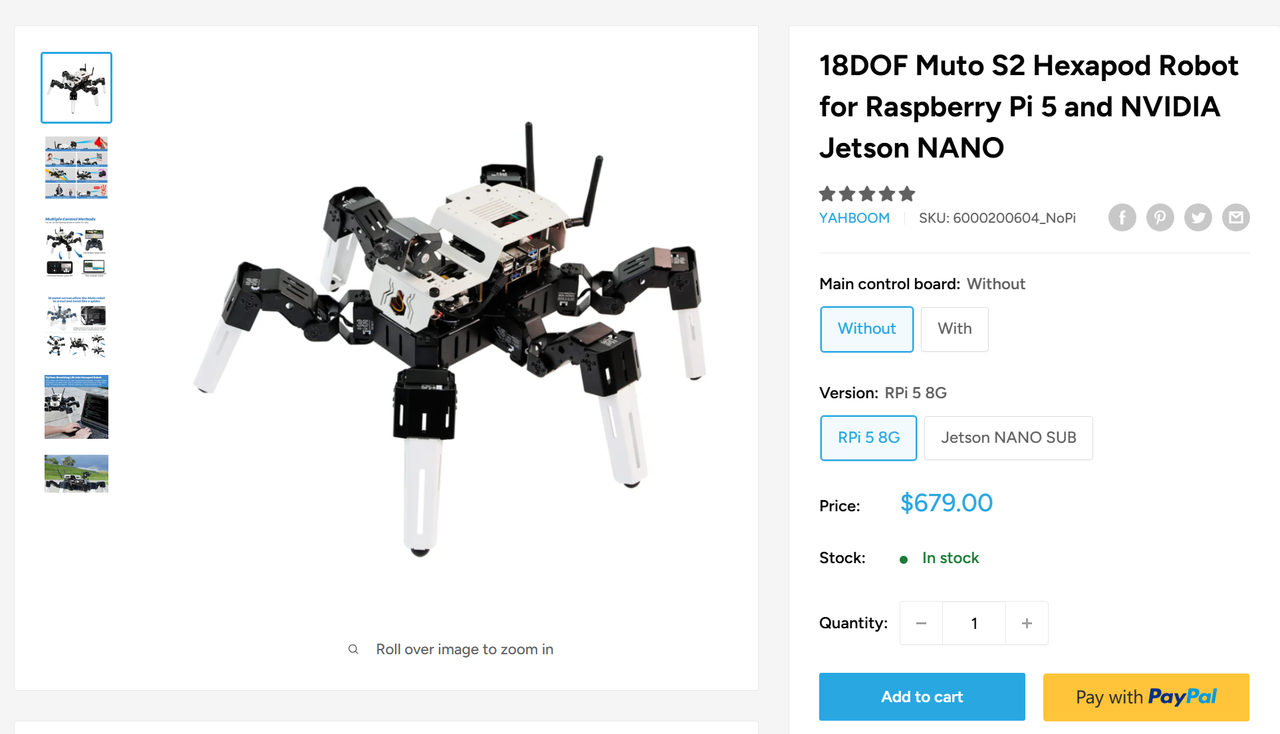
\includegraphics[width=0.3\linewidth]{pic/muto s2.PNG}
        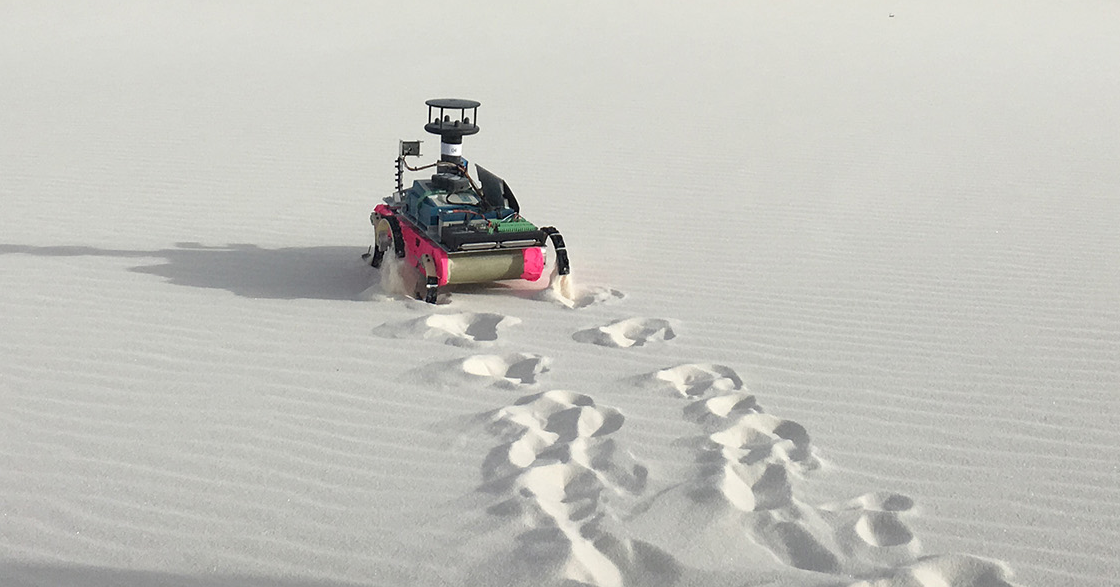
\includegraphics[width=0.3\linewidth]{pic/沙漠六足机器人.png}
        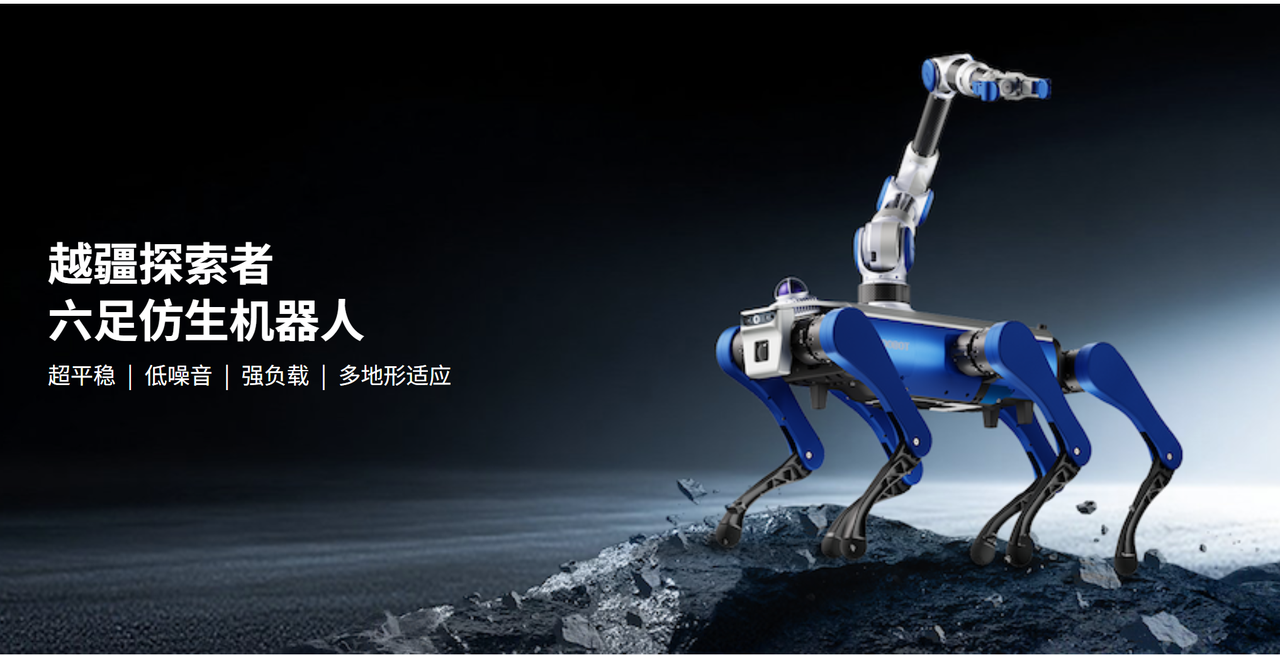
\includegraphics[width=0.3\linewidth]{pic/六足带机械臂狗.png}
    \end{figure}
\end{frame}

\begin{frame}{六足机器人避障的难点与研究动机}
    六足机器人在复杂环境下的自主避障,面临以下挑战:
    \begin{itemize}
        \item \textbf{姿态控制复杂}:六足机器人具有多个自由度,
              在避障过程中需要同时兼顾 \textbf{步态稳定性、能耗优化和绕障效率}。
        \item \textbf{视觉与控制耦合困难}:视觉传感器获取的环境信息
              存在 \textbf{延迟、噪声和不确定性},如何与实时步态调整协调仍是难题。
        \item \textbf{环境动态性强}:障碍物的形态与分布复杂,
              导致传统静态路径规划方法难以满足实时避障需求。
    \end{itemize}

    \vspace{0.3cm}
    \textbf{研究动机:}  
    本课题旨在探索 \textbf{六足机器人多足步态控制并实现避障}的方法,
    提升其在复杂环境下的避障能力与自主性。
\end{frame}

<<<<<<< HEAD
\section{前期研究}

\begin{frame}{六足机器人组装测试}
    目前已经实现:
    \begin{itemize}
        \item 六足机器人的手柄和局域网连接操控;
        \item 示例控制动作和摄像头的控制;
        \item 和Jetson Nano系统的连接。
    \end{itemize}
\end{frame}

\begin{frame}{六足机器人组装测试}
    \begin{figure}[htpb]
        \centering
        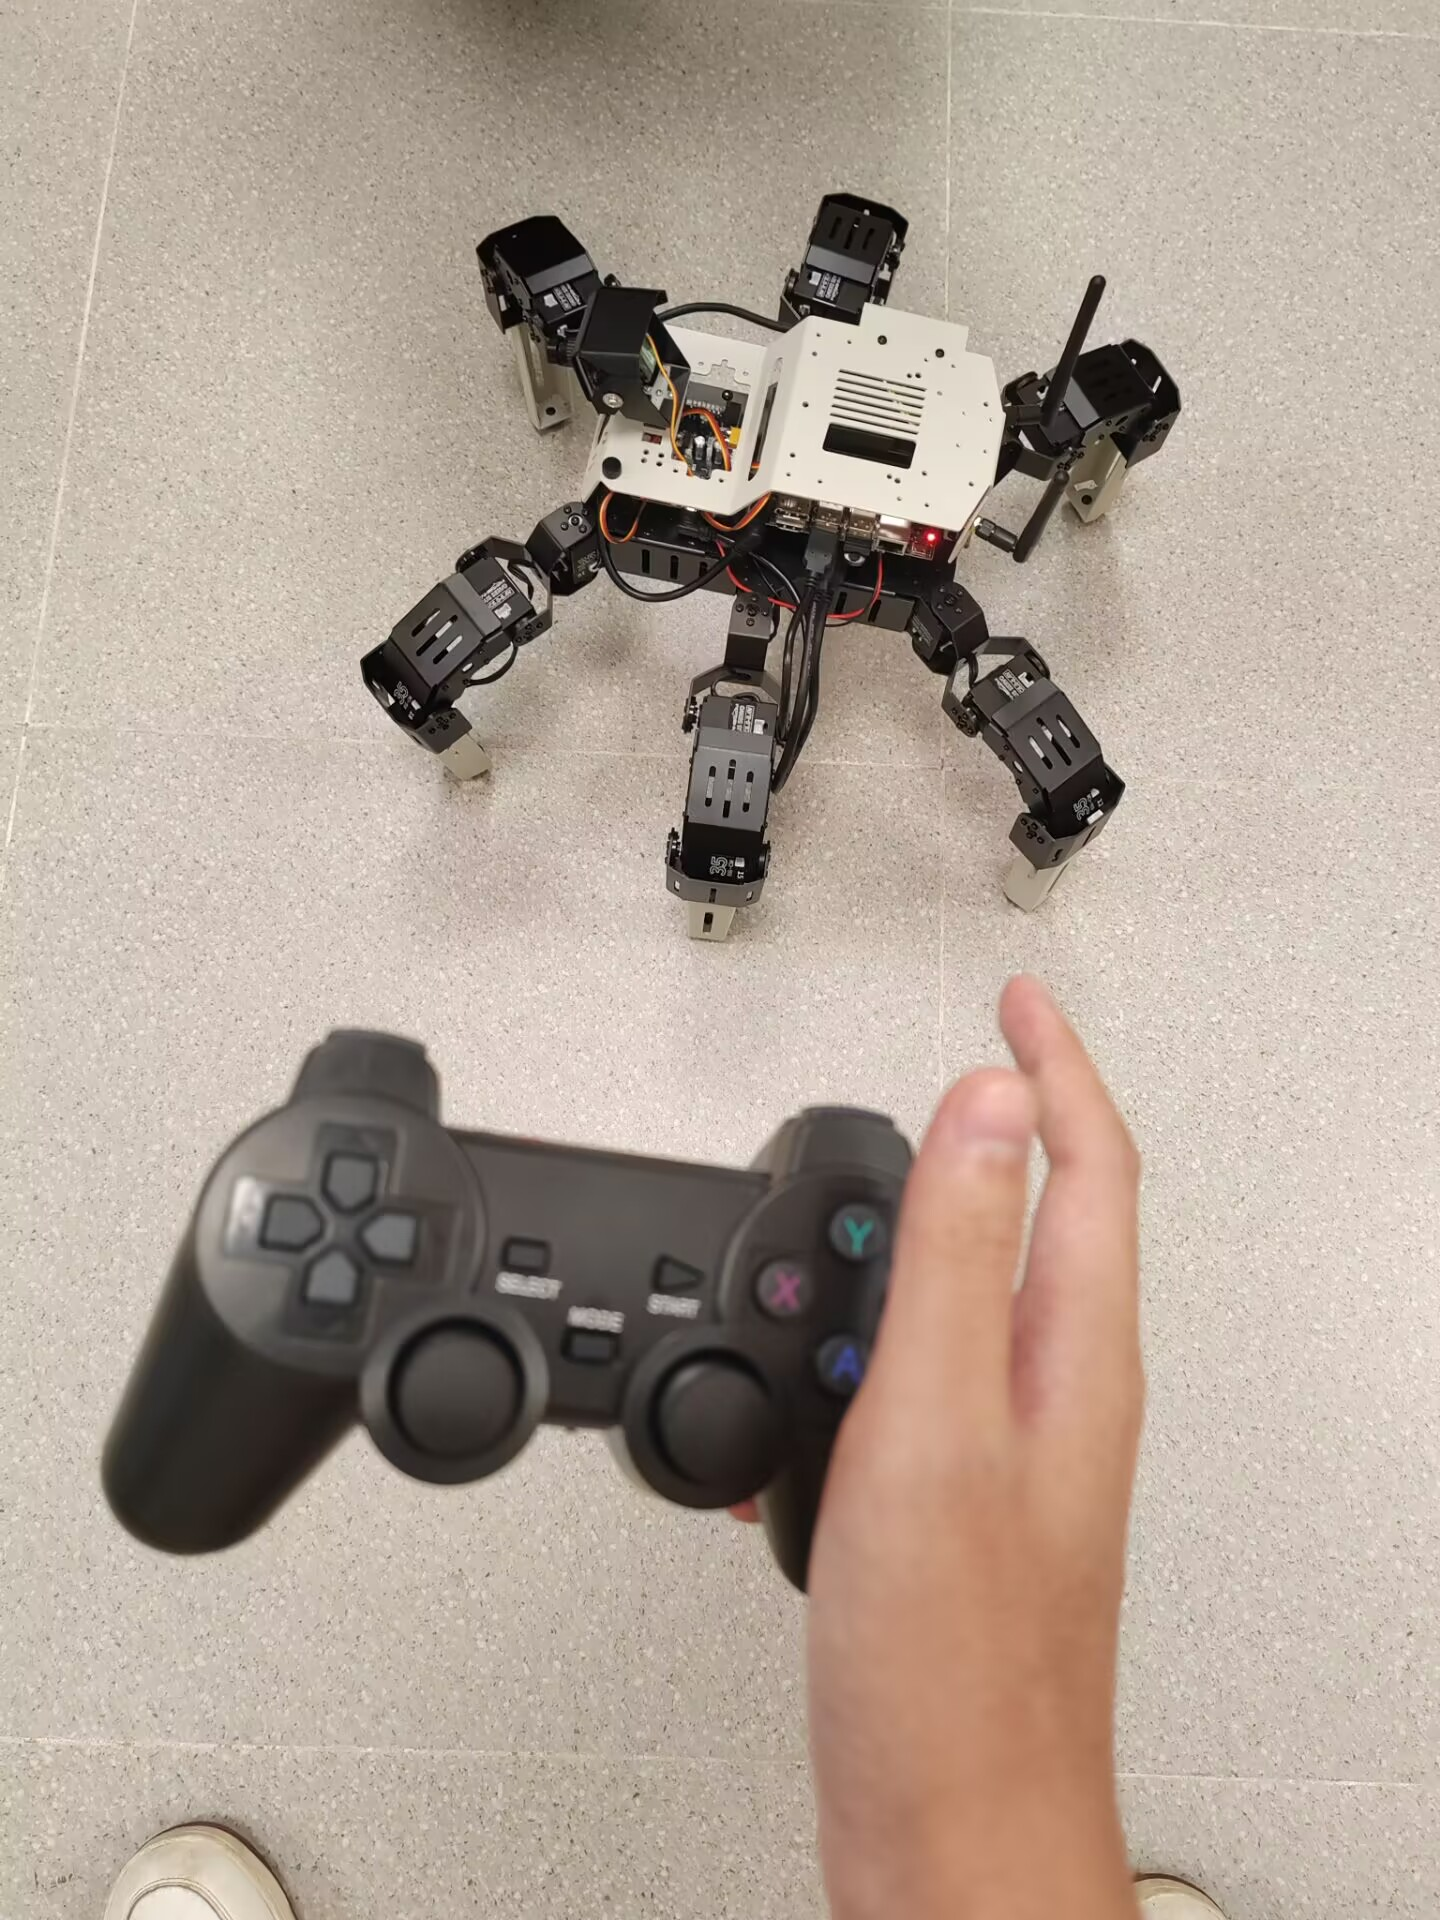
\includegraphics[width=0.49\linewidth]{pic/hex.jpg}
        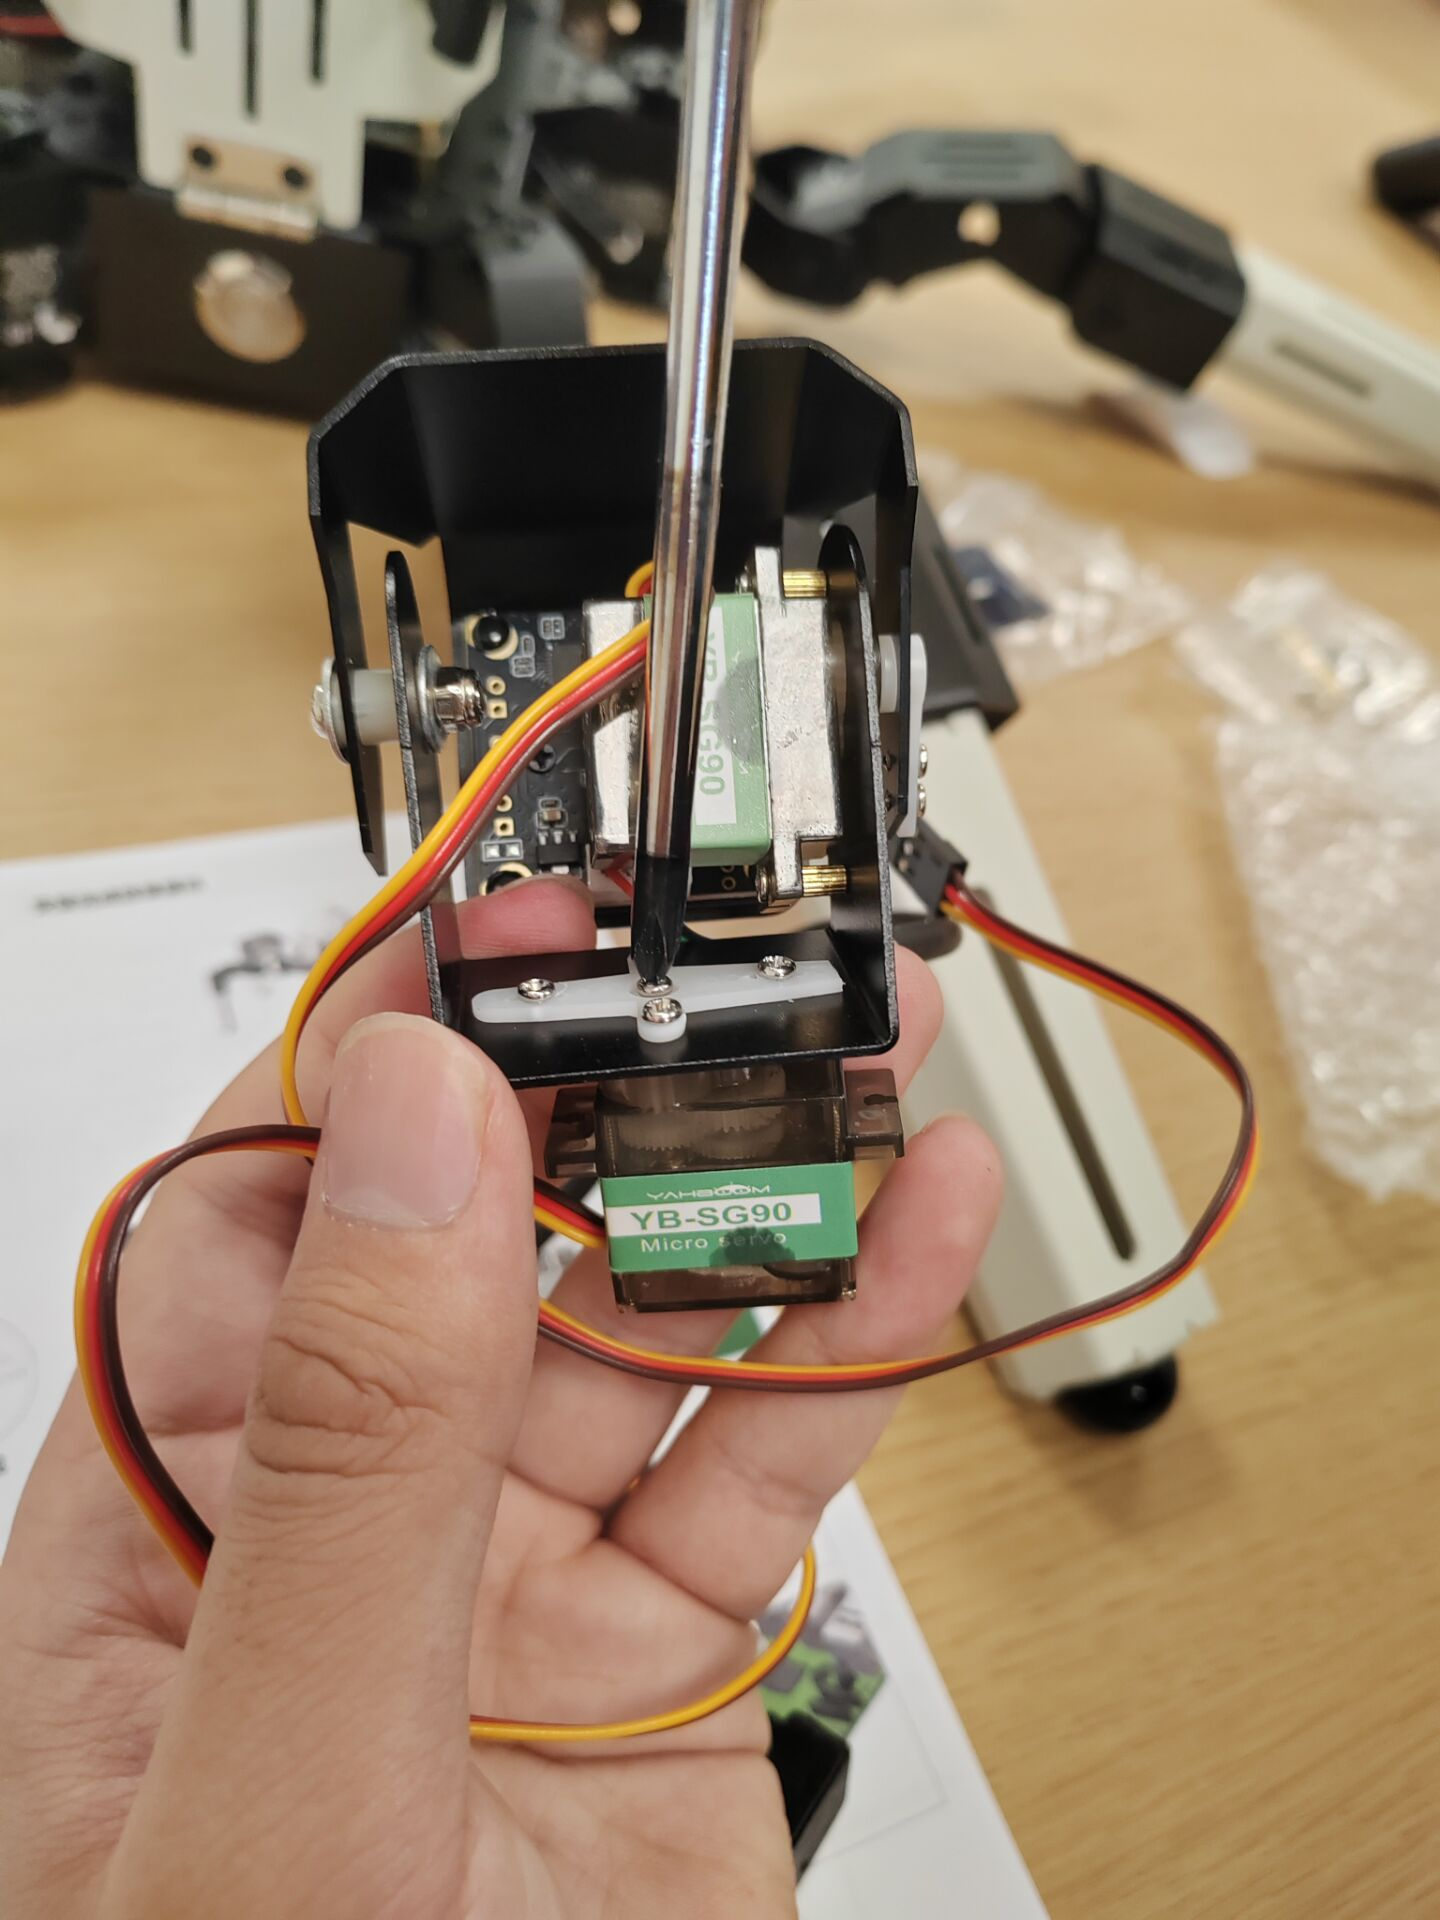
\includegraphics[width=0.49\linewidth]{pic/constr.jpg}
    \end{figure}
\end{frame}

\begin{frame}{六足机器人运动逻辑}
    \begin{itemize}
        \item 三角步态(Tripod Gait)
        \\ 六条腿分为两组(A组:1、4、5;B组:2、3、6)。一组支撑身体,另一组摆动向前。保证机器人始终有三条腿接触地面,保持稳定。
        \item 波浪步态(Wave Gait)
        \\ 六条腿依次抬起、摆动、落下,形成波浪推进。适合复杂地形。
    \end{itemize}
\end{frame}

\begin{frame}{六足机器人硬件架构}
    \begin{figure}[htpb]
        \centering
        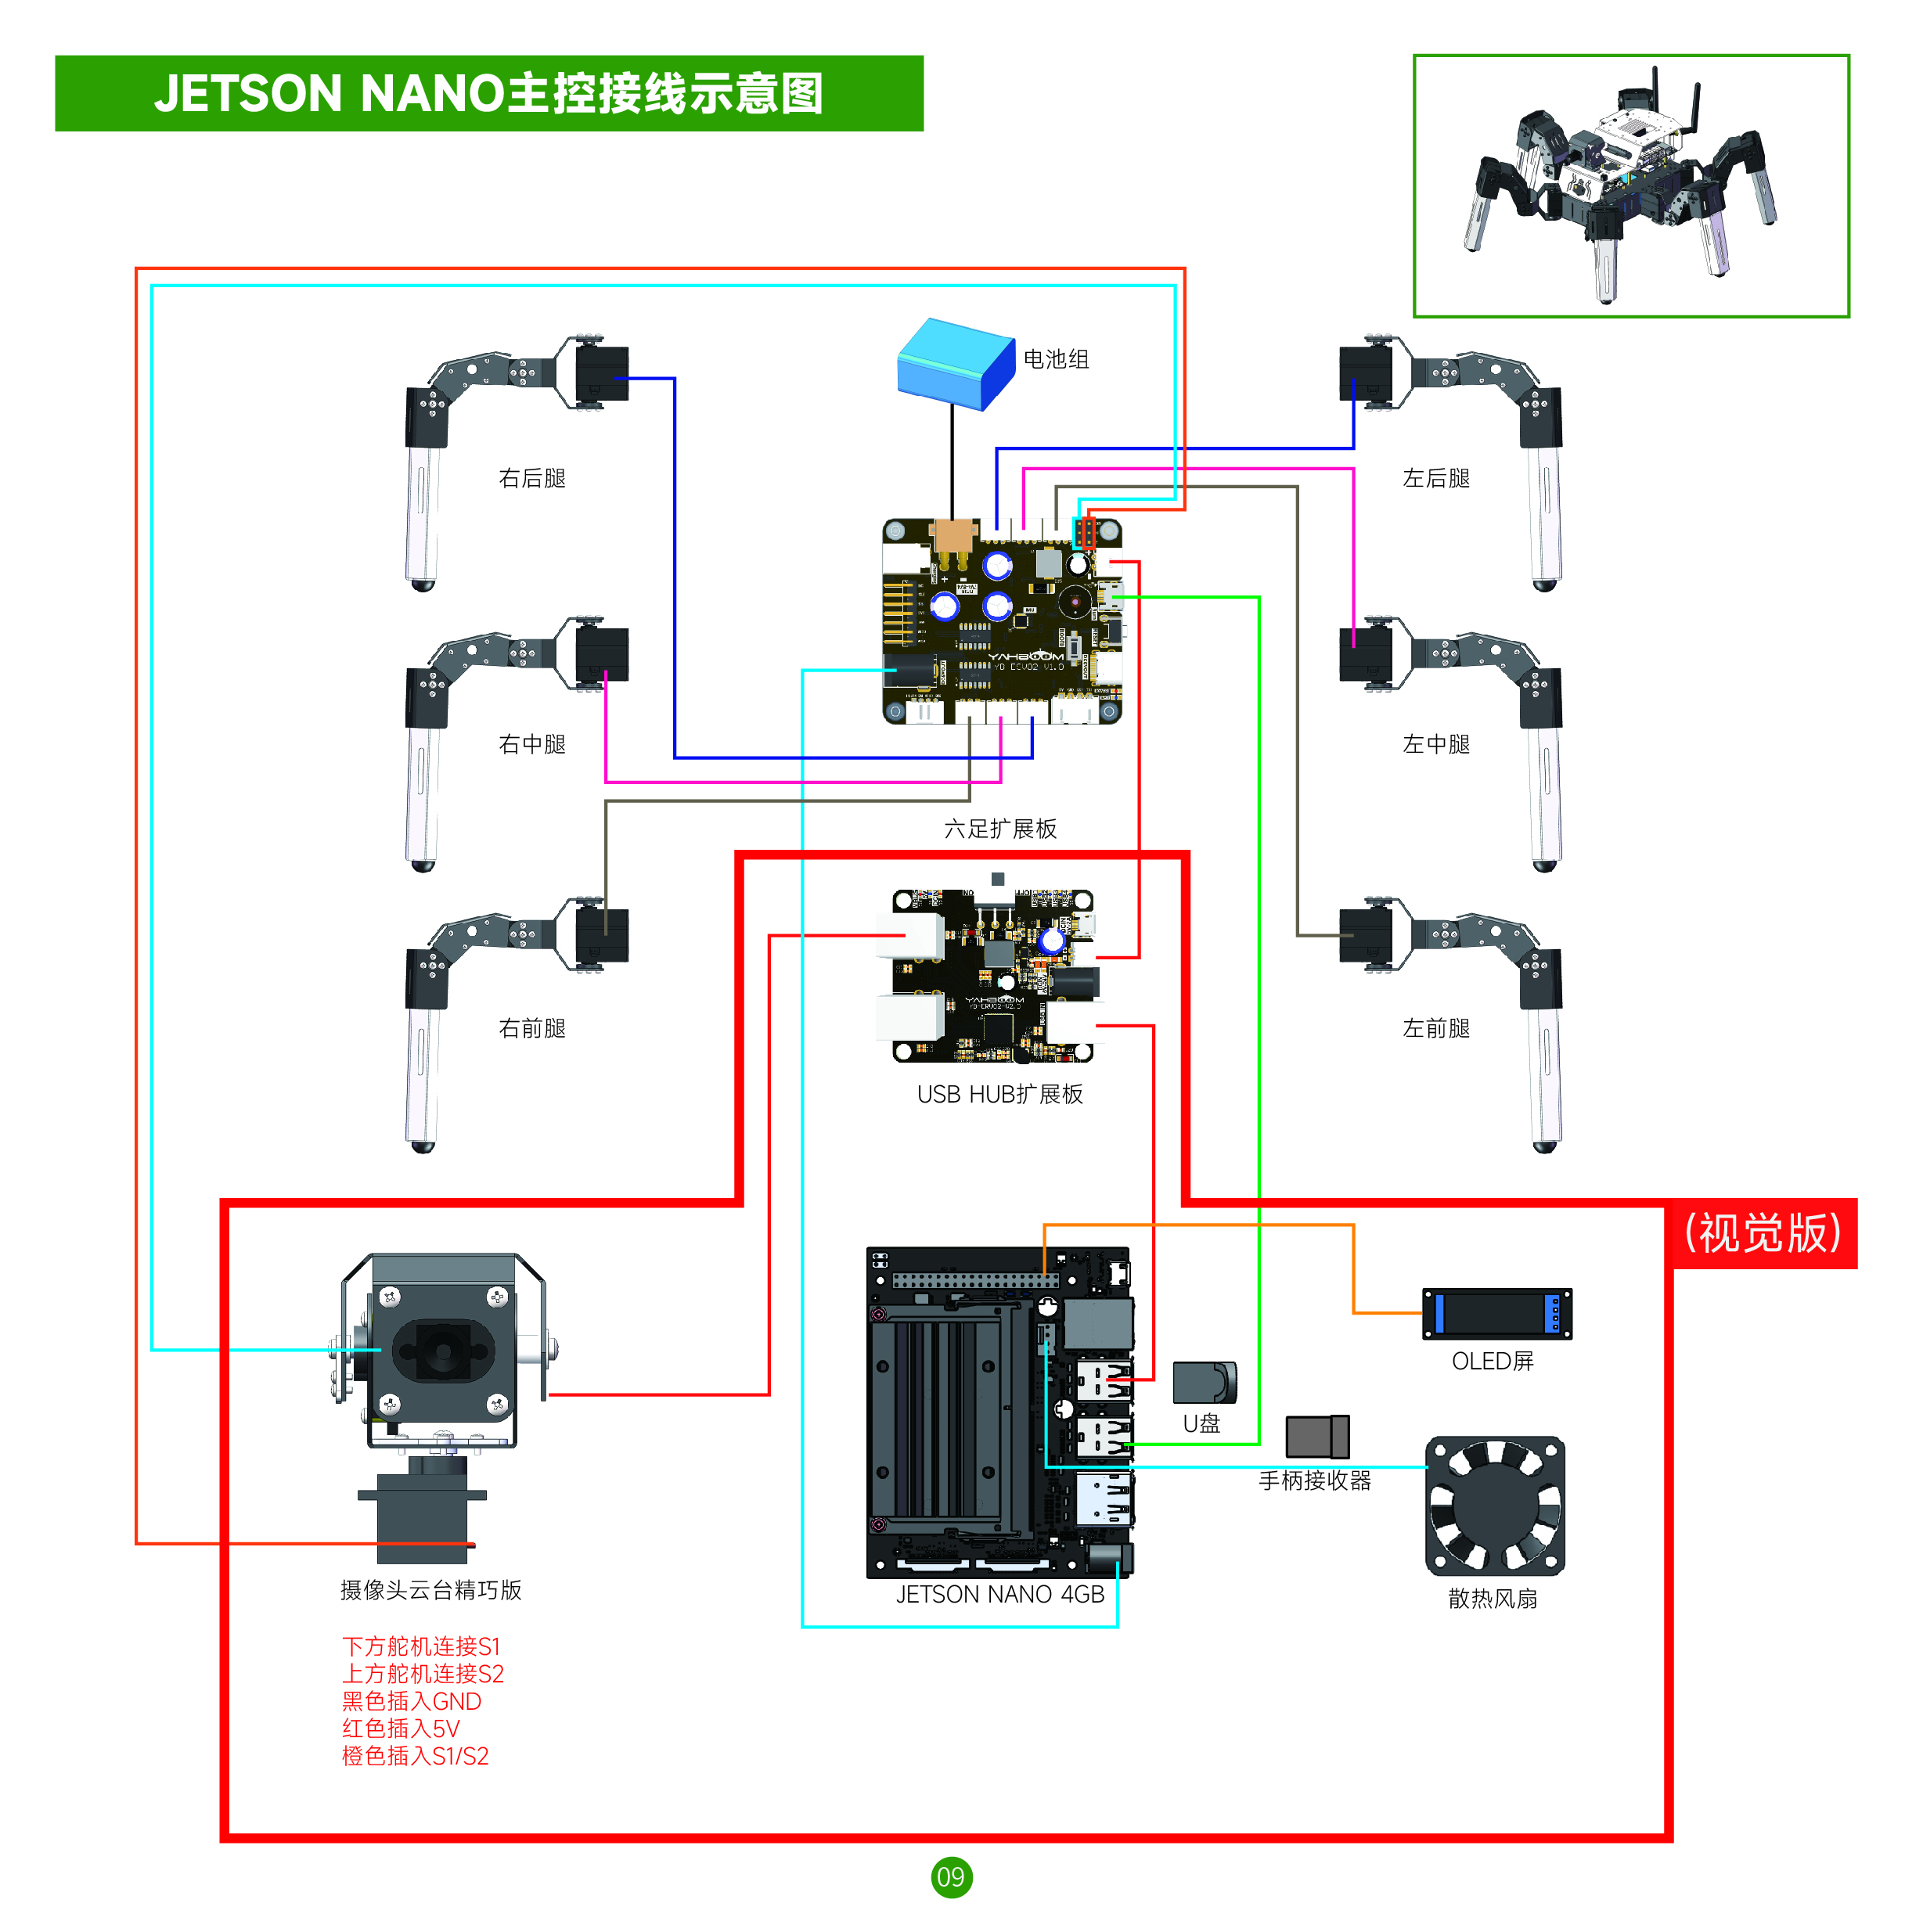
\includegraphics[width=0.6\linewidth]{pic/arch.jpg}
    \end{figure}
\end{frame}

\begin{frame}{六足机器人硬件架构}
    \begin{itemize}
        \item 顶层(Jetson Nano):
        \\ 负责路径规划、目标识别、避障算法、通信等功能,通过串口/总线将指令下发给STM32扩展板。Jetson Nano采用带桌面的Ubuntu作为操作系统。
        \item 底层(STM32控制板):
        \\ 负责PWM舵机驱动、步态切换、姿态保持、传感器数据读取等,通过预设的步态算法执行任务。
        \item 单腿硬件:
        \\ 每只腿包含3个舵机,分别是:肩关节(控制腿向前/后/侧方向摆动,决定运动方向(前进、转向、横移)),大腿关节(控制大腿的抬起和放下)和膝关节(控制小腿弯曲/伸直,影响步幅长度和对地形的适应性。)。
    \end{itemize}
\end{frame}

\begin{frame}{六足机器人软件架构}
    \begin{itemize}
        \item 人机输入层(操作者)
        \\ 输入设备:手柄 / 手机APP / 键盘 / 上位机 GUI(带摄像头流/深度视图)
        \item 上位控制层(Jetson Nano)
        \\ 接收人控指令、实时显示视频、将高层命令转为步态/动作模板 + 参数、发送到 STM32。使用Python/ROS 节点(推荐 ROS 或 socket 通信)。
        \item 步态规划与变换层(Jetson Nano或STM32)
        \\ 将“动作命令(如前进、左移、抬右前腿)”转为每条腿的期望足端轨迹(时序/位置/速度)。
        \item 逆运动学与舵机控制层(STM32)
        \\ 把足端轨迹转为 18 个舵机角度,通过 PWM/串口控制舵机;做低级 PID 或 P 控制。
    \end{itemize}
\end{frame}

\begin{frame}{六足机器人攀爬逻辑}
    需要更加精细的人机配合,将攀爬分解为多个动作:
    \begin{itemize}
        \item 靠近障碍物
        \\ 人控制机器人前进至台阶/障碍前。前腿抬高并落在台阶上。
        \\指令:前腿(1、2号腿) → 抬升(肩关节、大腿关节、膝关节配合)。后四条腿推动身体前移。中腿、后腿支撑,身体前压,重心前移。
        \item 中腿上台阶
        \\ 人依次控制中间的腿抬高,落在台阶上,前腿后腿支撑。
        \item 后腿跟随
        \\ 最后控制后腿抬高、上台阶,前腿,中腿支撑,恢复正常步态。
    \end{itemize}
    整个过程中,人像“指挥员”,根据障碍物高度和机器人姿态,逐条下达“抬腿、落腿、推身”的动作指令。且过程中,始终有4条腿在支撑,维持平衡。
\end{frame}

\section{后续研究计划}

% \subsection{Beamer主题分类}

\begin{frame}{研究计划与时间安排(前期:步态与避障,1--6周)}
    本课题基于 Yahboom Muto S2 六足机器人展开研究,前 6 周计划如下:
    \begin{itemize}
        \item \textbf{第1-2周}:Muto S2 六足机器人组装与调试(舵机校准、供电与通信测试)
        \item \textbf{第3周}:学习并运行官方示例代码,掌握基础步态调用方式
        \item \textbf{第4周}:自定义步态编写与调试,测试不同步态下的稳定性
        \item \textbf{第5周}:姿态控制机制研究(重心保持、步态切换、抗摆动策略)
        \item \textbf{第6周}:平地与低矮障碍环境下行走与避障实验,记录基线数据
        \item \textbf{第7周}:避障动作衔接优化,总结阶段性成果
    \end{itemize}
\end{frame}

\begin{frame}{研究计划与时间安排(后期:攀爬与总结,7--12周)}
    本课题的第 7--12 周重点在于攀爬功能实现与最终展示:
    \begin{itemize}
        \item \textbf{第7周}:攀爬功能需求分析与可行性评估(关节极限、力学约束、动作安全性)
        \item \textbf{第8周}:攀爬动作设计(支撑序列、重心迁移方案、步态与姿态组合)
        \item \textbf{第9-10周}:攀爬控制程序实现与初步调试(台阶/低矮平台)
        \item \textbf{第11周}:行走—避障—攀爬的动作衔接优化,综合实验
        \item \textbf{第12周}:实验数据分析,完成最终报告与答辩准备
    \end{itemize}
\end{frame}

% \section{研究内容}

% \subsection{美化主题}

% \begin{frame}{这一份主题与原始的THU Beamer Theme区别在于}
%     \begin{itemize}
%         \item 顶栏的小点变成一行而不是多行
%         \item 中文采用楷书
%         \item 剩下我改了啥我也忘了……我16年魔改的,都四年过去了(x
%         \item 更多该模板的功能可以参考 \url{https://www.latexstudio.net/archives/4051.html}
%         \item 下面列举出了一些Beamer的用法,部分节选自 \url{https://tuna.moe/event/2018/latex/}
%     \end{itemize}
% \end{frame}

% \subsection{如何更好地做Beamer}

% \begin{frame}{Why Beamer}
%     \begin{itemize}
%         \item \LaTeX 广泛用于学术界,期刊会议论文模板
%     \end{itemize}
%     \begin{table}[h]
%         \centering
%         \begin{tabular}{c|c}
%             Microsoft\textsuperscript{\textregistered}  Word & \LaTeX \\
%             \hline
%             文字处理工具 & 专业排版软件 \\
%             容易上手,简单直观 & 容易上手 \\
%             所见即所得 & 所见即所想,所想即所得 \\
%             高级功能不易掌握 & 进阶难,但一般用不到 \\
%             处理长文档需要丰富经验 & 和短文档处理基本无异 \\
%             花费大量时间调格式 & 无需担心格式,专心作者内容 \\
%             公式排版差强人意 & 尤其擅长公式排版 \\
%             二进制格式,兼容性差 & 文本文件,易读、稳定 \\
%             付费商业许可 & 自由免费使用 \\
%         \end{tabular}
%     \end{table}
% \end{frame}

% \begin{frame}{排版举例}
%     \begin{exampleblock}{无编号公式} % 加 * 
%         \begin{equation*}
%             J(\theta) = \mathbb{E}_{\pi_\theta}[G_t] = \sum_{s\in\mathcal{S}} d^\pi (s)V^\pi(s)=\sum_{s\in\mathcal{S}} d^\pi(s)\sum_{a\in\mathcal{A}}\pi_\theta(a|s)Q^\pi(s,a)
%         \end{equation*}
%     \end{exampleblock}
%     \begin{exampleblock}{多行多列公式\footnote{如果公式中有文字出现,请用 $\backslash$mathrm\{\} 或者 $\backslash$text\{\} 包含,不然就会变成 $clip$,在公式里看起来比 $\mathrm{clip}$ 丑非常多。}}
%         % 使用 & 分隔
%         \begin{align}
%             Q_\mathrm{target}&=r+\gamma Q^\pi(s^\prime, \pi_\theta(s^\prime)+\epsilon)\\
%             \epsilon&\sim\mathrm{clip}(\mathcal{N}(0, \sigma), -c, c)\nonumber
%         \end{align}
%     \end{exampleblock}
% \end{frame}

% \begin{frame}
%     \begin{exampleblock}{编号多行公式}
%         % Taken from Mathmode.tex
%         \begin{multline}
%             A=\lim_{n\rightarrow\infty}\Delta x\left(a^{2}+\left(a^{2}+2a\Delta x+\left(\Delta x\right)^{2}\right)\right.\label{eq:reset}\\
%             +\left(a^{2}+2\cdot2a\Delta x+2^{2}\left(\Delta x\right)^{2}\right)\\
%             +\left(a^{2}+2\cdot3a\Delta x+3^{2}\left(\Delta x\right)^{2}\right)\\
%             +\ldots\\
%             \left.+\left(a^{2}+2\cdot(n-1)a\Delta x+(n-1)^{2}\left(\Delta x\right)^{2}\right)\right)\\
%             =\frac{1}{3}\left(b^{3}-a^{3}\right)
%         \end{multline}
%     \end{exampleblock}
% \end{frame}

% \begin{frame}{图形与分栏}
%     % From thuthesis user guide.
%     \begin{minipage}[c]{0.3\linewidth}
%         \psset{unit=0.8cm}
%         \begin{pspicture}(-1.75,-3)(3.25,4)
%             \psline[linewidth=0.25pt](0,0)(0,4)
%             \rput[tl]{0}(0.2,2){$\vec e_z$}
%             \rput[tr]{0}(-0.9,1.4){$\vec e$}
%             \rput[tl]{0}(2.8,-1.1){$\vec C_{ptm{ext}}$}
%             \rput[br]{0}(-0.3,2.1){$\theta$}
%             \rput{25}(0,0){%
%             \psframe[fillstyle=solid,fillcolor=lightgray,linewidth=.8pt](-0.1,-3.2)(0.1,0)}
%             \rput{25}(0,0){%
%             \psellipse[fillstyle=solid,fillcolor=yellow,linewidth=3pt](0,0)(1.5,0.5)}
%             \rput{25}(0,0){%
%             \psframe[fillstyle=solid,fillcolor=lightgray,linewidth=.8pt](-0.1,0)(0.1,3.2)}
%             \rput{25}(0,0){\psline[linecolor=red,linewidth=1.5pt]{->}(0,0)(0.,2)}
% %           \psRotation{0}(0,3.5){$\dot\phi$}
% %           \psRotation{25}(-1.2,2.6){$\dot\psi$}
%             \psline[linecolor=red,linewidth=1.25pt]{->}(0,0)(0,2)
%             \psline[linecolor=red,linewidth=1.25pt]{->}(0,0)(3,-1)
%             \psline[linecolor=red,linewidth=1.25pt]{->}(0,0)(2.85,-0.95)
%             \psarc{->}{2.1}{90}{112.5}
%             \rput[bl](.1,.01){C}
%         \end{pspicture}
%     \end{minipage}\hspace{1cm}
%     \begin{minipage}{0.5\linewidth}
%         \medskip
%         %\hspace{2cm}
%         \begin{figure}[h]
%             \centering
%             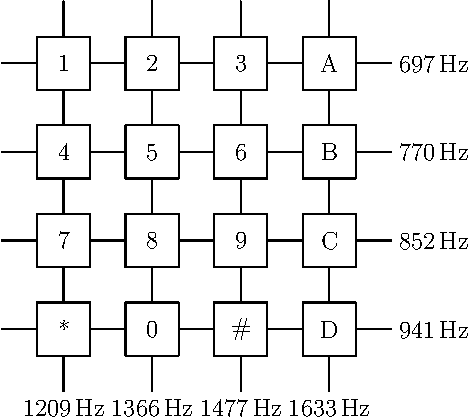
\includegraphics[height=.4\textheight]{pic/dtmf.pdf}
%         \end{figure}
%     \end{minipage}
% \end{frame}

% \begin{frame}[fragile]{\LaTeX{} 常用命令}
%     \begin{exampleblock}{命令}
%         \centering
%         \footnotesize
%         \begin{tabular}{llll}
%             \cmd{chapter} & \cmd{section} & \cmd{subsection} & \cmd{paragraph} \\
%             章 & 节 & 小节 & 带题头段落 \\\hline
%             \cmd{centering} & \cmd{emph} & \cmd{verb} & \cmd{url} \\
%             居中对齐 & 强调 & 原样输出 & 超链接 \\\hline
%             \cmd{footnote} & \cmd{item} & \cmd{caption} & \cmd{includegraphics} \\
%             脚注 & 列表条目 & 标题 & 插入图片 \\\hline
%             \cmd{label} & \cmd{cite} & \cmd{ref} \\
%             标号 & 引用参考文献 & 引用图表公式等\\\hline
%         \end{tabular}
%     \end{exampleblock}
%     \begin{exampleblock}{环境}
%         \centering
%         \footnotesize
%         \begin{tabular}{lll}
%             \env{table} & \env{figure} & \env{equation}\\
%             表格 & 图片 & 公式 \\\hline
%             \env{itemize} & \env{enumerate} & \env{description}\\
%             无编号列表 & 编号列表 & 描述 \\\hline
%         \end{tabular}
%     \end{exampleblock}
% \end{frame}

% \begin{frame}[fragile]{\LaTeX{} 环境命令举例}
%     \begin{minipage}{0.5\linewidth}
% \begin{lstlisting}[language=TeX]
% \begin{itemize}
%   \item A \item B
%   \item C
%   \begin{itemize}
%     \item C-1
%   \end{itemize}
% \end{itemize}
% \end{lstlisting}
%     \end{minipage}\hspace{1cm}
%     \begin{minipage}{0.3\linewidth}
%         \begin{itemize}
%             \item A
%             \item B
%             \item C
%             \begin{itemize}
%                 \item C-1
%             \end{itemize}
%         \end{itemize}
%     \end{minipage}
%     \medskip
%     \pause
%     \begin{minipage}{0.5\linewidth}
% \begin{lstlisting}[language=TeX]
% \begin{enumerate}
%   \item 巨佬 \item 大佬
%   \item 萌新
%   \begin{itemize}
%     \item[n+e] 瑟瑟发抖
%   \end{itemize}
% \end{enumerate}
% \end{lstlisting}
%     \end{minipage}\hspace{1cm}
%     \begin{minipage}{0.3\linewidth}
%         \begin{enumerate}
%             \item 巨佬
%             \item 大佬
%             \item 萌新
%             \begin{itemize}
%                 \item[n+e] 瑟瑟发抖
%             \end{itemize}
%         \end{enumerate}
%     \end{minipage}
% \end{frame}

% \begin{frame}[fragile]{\LaTeX{} 数学公式}
%     \begin{columns}
%         \begin{column}{.55\textwidth}
% \begin{lstlisting}[language=TeX]
% $V = \frac{4}{3}\pi r^3$

% \[
%   V = \frac{4}{3}\pi r^3
% \]

% \begin{equation}
%   \label{eq:vsphere}
%   V = \frac{4}{3}\pi r^3
% \end{equation}
% \end{lstlisting}
%         \end{column}
%         \begin{column}{.4\textwidth}
%             $V = \frac{4}{3}\pi r^3$
%             \[
%                 V = \frac{4}{3}\pi r^3
%             \]
%             \begin{equation}
%                 \label{eq:vsphere}
%                 V = \frac{4}{3}\pi r^3
%             \end{equation}
%         \end{column}
%     \end{columns}
%     \begin{itemize}
%         \item 更多内容请看 \href{https://zh.wikipedia.org/wiki/Help:数学公式}{\color{purple}{这里}}
%     \end{itemize}
% \end{frame}

% \begin{frame}[fragile]
%     \begin{columns}
%         \column{.6\textwidth}
% \begin{lstlisting}[language=TeX]
%     \begin{table}[htbp]
%       \caption{编号与含义}
%       \label{tab:number}
%       \centering
%       \begin{tabular}{cl}
%         \toprule
%         编号 & 含义 \\
%         \midrule
%         1 & 4.0 \\
%         2 & 3.7 \\
%         \bottomrule
%       \end{tabular}
%     \end{table}
%     公式~(\ref{eq:vsphere}) 的
%     编号与含义请参见
%     表~\ref{tab:number}。
% \end{lstlisting}
%         \column{.4\textwidth}
%         \begin{table}[htpb]
%             \centering
%             \caption{编号与含义}
%             \label{tab:number}
%             \begin{tabular}{cl}\toprule
%                 编号 & 含义 \\\midrule
%                 1 & 4.0\\
%                 2 & 3.7\\\bottomrule
%             \end{tabular}
%         \end{table}
%         \normalsize 公式~(\ref{eq:vsphere})的编号与含义请参见表~\ref{tab:number}。
%     \end{columns}
% \end{frame}

% \begin{frame}{作图}
%     \begin{itemize}
%         \item 矢量图 eps, ps, pdf
%         \begin{itemize}
%             \item METAPOST, pstricks, pgf $\ldots$
%             \item Xfig, Dia, Visio, Inkscape $\ldots$
%             \item Matlab / Excel 等保存为 pdf
%         \end{itemize}
%         \item 标量图 png, jpg, tiff $\ldots$
%         \begin{itemize}
%             \item 提高清晰度,避免发虚
%             \item 应尽量避免使用
%         \end{itemize}
%     \end{itemize}
%     \begin{figure}[htpb]
%         \centering
%         
\includegraphics[width=0.2\linewidth]{pic/whulogo.png}
%         \caption{这个校徽是标量图,找不到矢量图捏}
%     \end{figure}
% \end{frame}

% \section{计划进度}
% \begin{frame}
%     \begin{itemize}
%         \item 一月:完成文献调研
%         \item 二月:复现并评测各种Beamer主题美观程度
%         \item 三、四月:美化THU Beamer主题
%         \item 五月:论文撰写
%     \end{itemize}
% \end{frame}

% \section{参考文献}

% \begin{frame}[allowframebreaks]
%     \bibliography{ref}
%     \bibliographystyle{alpha}
%     % 如果参考文献太多的话,可以像下面这样调整字体:
%     % \tiny\bibliographystyle{alpha}
% \end{frame}

\begin{frame}
    \begin{center}
        {\Huge\calligra Thanks!}
    \end{center}
\end{frame}

\end{document}